\paragraph{Definition}
We want a function $g$ that makes $RSS=\su{{i=1}}{n}\left(y_{i}-
g(x_{i})\right)^{2}$ small but also with constraint on $g(x_{i})$
therewith to avoid overfitting and get smooth curve.\\
A natural approach is to find the function $g$ that minimizes:
\begin{center}
	\encV{$\underbrace{\su{{i=1}}{n}\left(y_{i}-g(x_{i})\right)^{2}}_\text{Loss function}+\underbrace{\lambda\Su{}{} g''(t)^{2}dt}_\text{Penalty term}$}
\end{center}
where $\lambda$ is a nonnegative \emph{tunning parameter}, and $g$ is
a \tR{\emph{smoothing spline}}.\\

The first derivative $g'(t)$ measures the slope of a function at $t$,
and the second derivative corresponds to the amount by which the slope
is changing, \tR{if $g(t)$ is very wiggly near $t$ $g''(t)$ is large,
otherwise it is close to zero.}\\
$\Su{}{}g''(t)^{2}dt$ \sB{is a measure of the total change in the
function $g'(t)$, over its entire range}.
Since the solution is a natural spline, we can write is as:
\begin{center}
	\enc{ $ f(x)=\su{{j=1}}{N}N_{j}(x)\theta_{j}$}
\end{center}
where the \sB{$N_{j}(x)$ are a $N-\text{dimensional}$ set of basis functions} for representing this
family of natural splines:
$$ RSS(\theta, \lambda) = \left(\bm{y}-\bm{N}\theta\right)^{T}\left(\bm{y}-\bm{N}\theta\right) +
\lambda\theta^{T}\Omega_{N}\theta$$ where 
$\begin{cases}
\left\{N\right\}_{ij} = N_{j}(x_{i})\\
\left\{\Omega_{N}\right\}_{jk} = \Su{}{}N_{j}^{''}(t)N_{k}^{''}(t)dt
\end{cases}$
The solution is easily seen to be:
\begin{center}
	\encB{$ \hat{\theta} = \left(\bm{N}^{T}\bm{N} + \lambda\Omega_{N}\right)^{-1}\bm{N}^{T}$}
\end{center}
The fitted smoothing spline is given by:
$$\hat{f}(x)=\su{{j=1}}{N}\bm{N}_{j}(x)\hat{\theta}_{j}$$

\paragraph{Choosing the smoothing parameter $\lambda$}
\tB{The vector of fitted values, when applying a smoothing spline to 
the data, can be written as $n\times n$ matrix $S_{\lambda}$ times the 
response $y$}:
\begin{center}
$\hat{g}_{\lambda}=S_{\lambda}y$
\end{center}
where $\hat{g}$ is a smoothing spline for a particular choice of 
$\lambda$, that is it is a $n$-vector containing the fitted values of 
the smoothing spline at the training points $\prth{x}{i}{n}$\\

\begin{python}
import csaps
from csaps import csaps

kf = KFold(n_splits=5)
df2 = df.iloc[:, [0, 1]].groupby(df.columns[1]).agg(
    np.median).reset_index()
cv_dict = {str(i):0 for i in range(0, 100+1, 1)}
for k in range(0, 100+1, 1):
    mse_list = []
    for train, test in kf.split(df2.budget_std):
        smoothing_spline = csaps(df2.iloc[train, 1],
                                 df2.iloc[train, 0],
                                 smooth=round(k/100, 2))
        mse = ((smoothing_spline(
            df2.iloc[test, 0])-df2.iloc[test, 1])**2).mean()
        mse_list.append(mse)
    cv_dict[str(k)] = np.array(mse_list).mean()
cv_list = list({k:v for k,v in sorted(cv_dict.items(), key=lambda item: item[1])})

smoothing_spline = csaps(df2.iloc[:, 1], df2.iloc[:, 0],
                         smooth=round(float(cv_list[0])/100, 2))
# Create spline line for 50 evenly spaced values of age
xp = np.linspace(df2.iloc[:, 1].min(), df2.iloc[:, 1].max(), 50)
yp = smoothing_spline(xp)
\end{python}

\paragraph{Degrees of freedom refer to the number of free parameters} such as
the number of coefficients fit in a polynomial or cubic spline. Denote by $\hat{f}$ the 
$N-\text{vector}$ of fitted values $\hat{f}(x_{i})$ at the training predictors $x_{i}$:
\begin{align*}
	\hat{f}=&\bm{N}\left(\bm{N}^{T}\bm{N}+\lambda\bm{\Omega}_{N}\right)^{-1}\bm{N}^{T}\bm{y}\\
	=& \bm{S}_{\lambda}\bm{y}
\end{align*}
The finite linear operator \tB{$\bm{S}_{\lambda}$} is known as the \tB{\textit{smoother matrix}}\\
Linear operator are familiar in more traditional least squares fitting as well, suppose 
$B_{\zeta}$ is a $N\times M$ matrix of $M$ cubic-spline basis functions evaluated at the $N$
training points $x_{i}$, with knot sequence $\zeta$ and $M\ll N$. Then the vector of fitted spline
values is given by:
\begin{align*}
	\hat{f}=&\bm{B}_{\zeta}\left(\bm{B}_{\zeta}^{T}\bm{B}_{\zeta}\right)^{-1}\bm{B}_{\zeta}^{T}\bm{y}\\
	=& \bm{H}_{\zeta}\bm{y}
\end{align*}
The linear operator $\bm{H}_{\zeta}$ is a projection operator, also known as the \textit{hat 
matrix}.
\begin{itemize}
	\item Both $\bm{H}_{\zeta}\text{ and }\bm{S}_{\lambda}$ are symmetric, positive 
		semi-definite
	\item $\bm{H}_{\zeta}\bm{H}_{\zeta} = \bm{H}_{\zeta}$ (\textit{idempotent})\\
		$\bm{S}_{\lambda}\bm{S}_{\lambda}\preceq\bm{S}_{\lambda}$ 
		meaning that the right-hand side exceeds the left-hand by a positive semi-definite
		matrix. This is a consequence of the shrinking nature of $\bm{S}_{\lambda}$
	\item $\bm{H}_{\zeta}$ has rank $M$, while $\bm{S}_{\lambda}$ has rank $N$.
\end{itemize}
The expression $M = trace\left(\bm{H}_{\zeta}\right)$ gives the dimension of the projection
space, which is also the number of basis functions, and hence the number of parameters involved
in the fit. \\ By analogy we define the \textit{effective degrees of freedom} of a smoothing
spline to be: 

\sB{It is possible to show that as $\lambda$ increases from 0 to 
$\infty$, the effective degrees of freedom, which we write 
$df_{lambda}$, decreases from $n$ to 2}.\\
Hence $df_{\lambda}$ is a measure of the flexibility.
\begin{center}
	\encV{$df_{\lambda}=trace(\bm{S}_{\lambda})=\su{{i=1}}{n}\left\{ S_{\lambda}
	\right\}_{ii}$}
\end{center}
the sum of the diagonal elements of the matrix $S_{\lambda}$\\
Since $\bm{S}_{\lambda}$ is symmetric (and positive semi-definite), it has a real 
eigen-decomposition. Before we proceed, it is convenient to rewrite $\bm{S}_{\lambda}$ in the
\textit{Reinsch} form: $\bm{S}_{\lambda} = \left(\bm{I}+\lambda\bm{K}\right)^{-1}$ where $K$
does not depend on $\lambda$. Since $\hat{\bm{f}}=\bm{S}_{\lambda}\bm{y}$ solves: 
$\min\limits_{f}(\bm{y}-\bm{f})^{T}(\bm{y}-\bm{f})+\lambda\bm{f}^{T}\bm{K}\bm{f}$
The eigen-decomposition of $\bm{S}_{\lambda}$ is:
$$ \bm{S}_{\lambda}=\su{{k=1}}{N}\rho_{k}(\lambda)\bm{u}_{k}\bm{u}_{k}^{T}$$ with 
$\rho_{k}(\lambda)=\dfrac{1}{1+\lambda d_{k}}$ and $d_{k}$ the corresponding eigenvalue of $K$.

\tB{It turns out that the \emph{leave-cross-out} cross-validation error
(LOOCV) can be computed very efficiently for smoothing splines}, with
essentially the same cost as computing a single fit using the following
formula:
$$
RSS_{cv}(\lambda)=\su{{i=1}}{n}\left( y_{i}-\hat{g}_{\lambda}^{(-i)}(x_{i}) \right)^{2}=\su{{i=1}}{n}\left[ \dfrac{y_{i}-\hat{g}_{\lambda}(x_{i})}{1-\left\{ S_{\lambda} \right\}_{ii}} \right]^{2}
$$
The notation \tB{$\hat{g}_{\lambda}^{(-i)}(x_{i})$ indicates the fitted
value for this smoothing spline evaluated at $x_{i}$}, where the fit
uses all of the training observations except for the $i^{th}$
observation $(x_{i},y_{i})$. In contrast \tB{{$\hat{g}_{\lambda}(x_{
i})$ indicates the smoothing spline function fit to all of the training
observations and evaluated in $x_{i}$}}.

\paragraph{Automatic Selection of the Smoothing Parameters}
\subparagraph{The Bias-Variance Tradeoff}
\begin{align*}
	Cov\left(\hat{f}\right) =& Cov\left(\bm{S}_{\lambda}\bm{y}\right)\\
	=& \bm{S}_{\lambda} Cov\left(\bm{y}\right)\bm{S}_{\lambda}^{T}\\
	=& \bm{S}_{\lambda}\bm{S}_{\lambda}^{T}
\end{align*}
The diagonal contains the pointwise variances at the training $x_{i}$. The bias is given by:
\begin{align*}
	\text{Bias}(\hat{\bm{f}}) =& \bm{f} - \E{\hat{\bm{f}}}\\
	=& \bm{f} - \bm{S}_{\lambda}\bm{f}
\end{align*}
The integrated squared prediction error (EPE) combines both bias and variance in a single 
summary:
\begin{align*}
	EPE\left(\hat{f}_{\lambda}\right) =& \E{Y-\hat{f}_{\lambda}(X)}^{2}\\
	=& \V{Y}+\E{\text{Bias}^{2}\left(\hat{f}_{\lambda}(X)\right)+\V{\hat{f}_{\lambda}\left(X \right)}}\\
	=& \sigma^{2} + \text{MSE}\left(\hat{f}_{\lambda}\right)
\end{align*}

\subsection{Multidimensional Splines}

Suppose $X\in\mathbb{R}^{2}$ and we have a basis of functions $h_{1k}(X_{1})$ with $k\in\inter{1}{
M_{1}}$ for representing functions of coordinate $X_{1}$, and likewise a set of $M_{2}$ functions
$h_{2k}(X_{2})$ for coordinate $X_{2}$. Then the $M_{1}\times M_{2}$ dimensional \textit{tensor
product basis} defined by:
$$ g_{jk}(X) = h_{1j}(X_{1})h_{2k}(X_{2})\text{ with }(j,k)\in\inter{1}{M_{1}}\times\inter{1}{M_{
1}}$$ can be used for representing a $2-\text{dimensional}$ function: 
$$g(X)=\su{{j=1}}{M_{1}}\su{{j=1}}{M_{2}}\theta_{jk}g_{jk}(X)$$

\begin{figure}[H]
	\begin{center}
		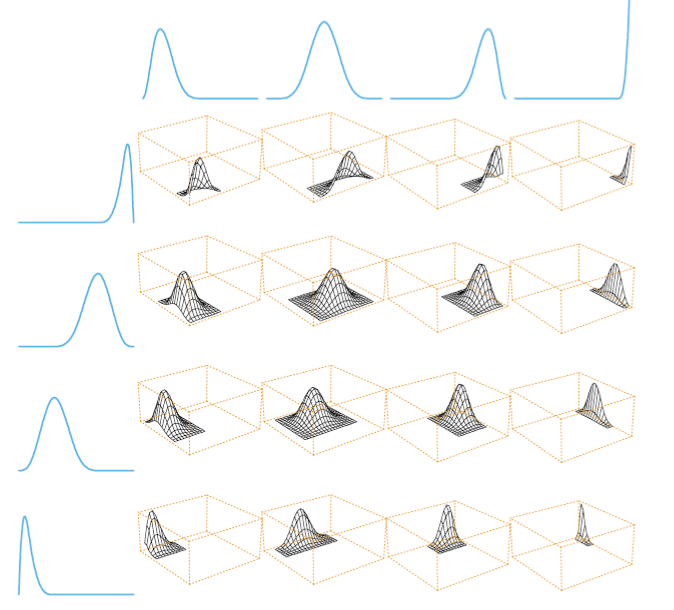
\includegraphics[width=\textwidth]{./chap/1chap/3sec/8images/2_tensorProduct.PNG}
	\end{center}
	\caption{A tensor product basis of $B-\text{splines}$, showing some selected pairs. Each
	$2-$dimensionnal function is the tensor product of the corresponding one dimension 
	marginals}
	\label{fig: 2_tensorProduct.PNG}
\end{figure}

\subsection{Wavelet Smoothing}
Wavelet typically use a complete orthonormal basis to represent functions, bu then shrink and 
select the coefficients toward a sparse representation.
\begin{figure}[H]
	\begin{center}
		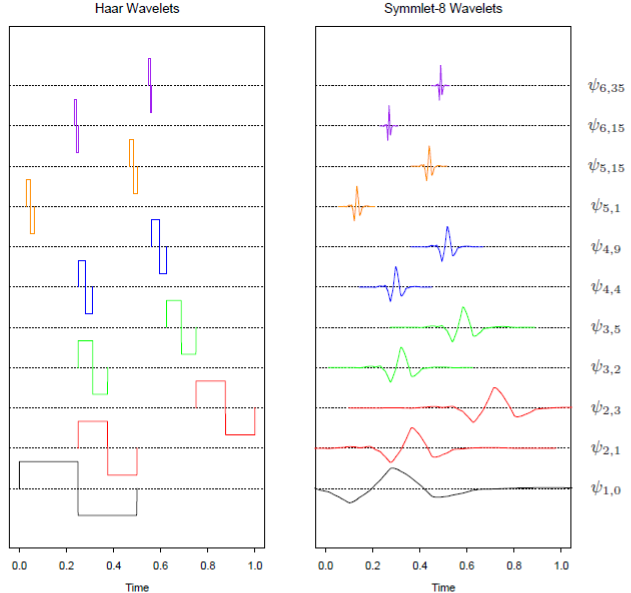
\includegraphics[width=\textwidth]{./chap/1chap/3sec/8images/3_wavelet.PNG}
	\end{center}
	\caption{Some selected wavelets at different translations and dilatations for the Haar
	and symmlet families. The functions have been scaled to suit the display.}
	\label{fig: 3_wavelet.PNG}
\end{figure}

\paragraph{Wavelet Bases and the Wavelet Transform}
Wavelet bases are generated by translations and dilatations of a single scaling function
$\phi(x)$ (also known as the \textit{father}).\\
The \textit{Haar} basis produces a piecewise-constant representation, thus if $\phi(x)=I(x\in
[0,1])$, then $\phi_{0,k}(x) = \phi(x-k)$, k an integer, generates an orthonormal basis for 
functions with jumps at the integrs. Call this reference space $V_{0}$\\
The dilatations $\phi_{1,k}(x)=\sqrt{2}(2x-k)$ form an orthonormal basis for a space 
$V_{1} \supset V_{0}$. More generally we have $\cdots \supset V_{1}\supset V_{1}\supset V_{1}
\supset \cdots$ where each $V_{j}$ is spanned by $\phi_{j,k}=2^{\frac{j}{2}}\phi(2^{j}x-k)$\\
We might represent a function in $V_{j+1}$ by a component in $V_{j+1}$ plus the component in
the orthogonal complement $W_{j}$ of $V_{j}$ to $V_{j+1}$ written as $V_{j+1}= V_{j}\bigoplus W_{j}$
The component in $W_{j}$ represents detail, and we might wish to set some elements of this 
components to zero. It is easy to see that the functions $\psi(x-k)$ generated by the 
\textit{mother wavelet} $\psi(x)=\phi(2x)-\phi{2x-1}$ form an orthonormal basis for $W_{0}$ for
the Haar family. Likewise $\psi_{j,k}=2^{\frac{j}{2}}\psi(2^{j}x-k)$ form a basis for $W_{j}$

Now $V_{j+1}=V_{j}\bigoplus W_{j} = V_{j-1}\bigoplus W_{j-1} \bigoplus W_{j}$, more generally:
$V_{j} = V_{0} \bigoplus W_{0} \bigoplus W_{1}\cdots W_{j-1}$. Notice that since these spaces
are orthogonal, all the basis functions are orthonormal. In fact, if the domain is discrete with 
$N=2^{J}$ (time) points, this is as far as we can go. 

\paragraph{Adaptive Wavelet Filtering}
Suppose $\bm{y}$ is the response vector, and $\bm{W}$ is the $N\times N$ orthonormal wavelet
basis matrix evaluated at the $N$ uniformly spaced observations. Then $\bm{y}^{*}=\bm{W}^{T}\bm{y}$
is called the \textit{wavelet transform} of $\bm{y}$\\
A popular method for adaptive wavelet fitting is known as SURE(Stein Unbiased Risk Estimation)
shrinkage, we start with the criterion:
$$ \min\limits_{\theta}\norm{\bm{y}-\bm{W}\bm{\theta}}_{2}^{2} + 2\lambda\norm{\theta}_{1}$$
Because $\bm{W}$ is orthonormal, this leads to the simple solution:
$$\hat{\theta}_{j} = sign(y_{i}^{*})(|y_{j}^{*}|-\lambda)_{+}$$
The least squares coefficient are translated toward zero, and truncated at zero.
The fitted function is then given by the \textit{inverse wavelet transform} $\hat{\bm{f}}=\bm{W\hat{\theta}}$

\subsection{Kernel Smoothing Methods}
We will describe a class of regression techniques that achieve flexibility  in estimating the 
regression function $f(X)$ over the domain $\mathbb{R}^{p}$ by \sB{fitting a different but simple
model separately at each query point $x_{0}$. This is done by using only those observations close
to the target point $x_{0}$ to fit the simple model}, and in such a way that the resulting 
estimated function $\hat{f}(X)$ is \textit{smooth} in $\mathbb{R}^{p}$\\ This \sB{localization is
achieved via a weighting function or kernel $K_{\lambda}(x_{0},x_{i})$}, which assigns a weight 
to $x_{i}$ based on its distance from $x_{0}$.

\paragraph{One-Dimensional Kernel Smoother }
\begin{figure}[H]
	\begin{center}
		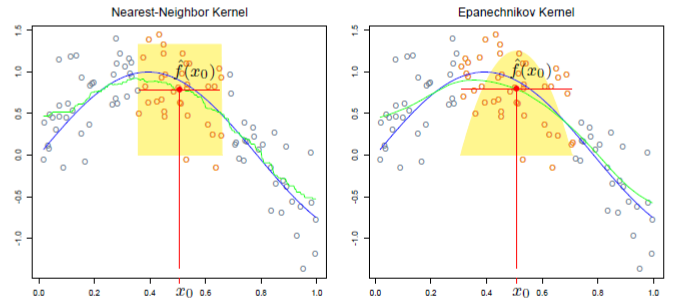
\includegraphics[width=\textwidth]{./chap/1chap/3sec/8images/40_localReg.PNG}
	\end{center}
	\caption{Left pannel is the result of a 30-nearest-neighbor running-mean smoother. The
	right panel is the result of a kernel-weighted average using \textit{Epanechnikov} kernel
	with (half) window width $\lambda=0.2$}
	\label{fig:40_localReg.PNG}
\end{figure}
The green curve is bumpy, since $\hat{f}(x)$ is discontinuous in $x$. As we move $x_{0}$ from left
to the right, the \emph{k}-nearest neighborhood remains constant, until a point $x_{i}$ to the right
of $x_{0}$ becomes closer than the furthest point $x_{i'}$ in the neighborhood to the left of 
$x_{0}$ at which time $x_{i}$ replaces $x_{i'}$.\\
\tB{Rather than give all the points in the neighborhood equal weight, we can assign weights that 
die off smoothly with distance from the target point as the so-called Nadaraya-Watson 
kernel-weighted average}:
\begin{center}
	\enc{$ \hat{f}(x_{0})=\dfrac{\su{{i=1}}{N}K_{\lambda}(x_{0},x_{i})y_{i}}{\su{{i=1}}{N}K_{\lambda}(x_{0},x_{i})}$}
\end{center}
with the \tB{\textit{Epanechenikov}} quadratic kernel:
$$ K_{\lambda}(x_{0}, x)=D\left(\dfrac{|x-x_{0}|}{\lambda}\right)\text{, with }D(t)=
\begin{cases}
	\frac{3}{4}(1-t^{2})\text{ if }|t|\leq 1\\
	0\text{ otherwise}
\end{cases}
$$
We can use such adaptive neighborhoods with kernels, more generally: 
\begin{center}
	\tR{$ K_{\lambda}(x_{0}, x)=D\left(\dfrac{|x-x_{0}|}{h_{\lambda}(x_{0})}\right)$}
\end{center}
\paragraph{Local Linear Regression}
Locally-weighted averages can be badly biased on the boundaries of the domain.
\begin{figure}[H]
	\begin{center}
		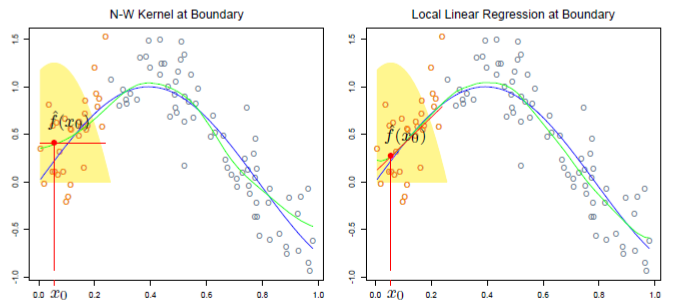
\includegraphics[width=\textwidth]{./chap/1chap/3sec/8images/4_localReg.PNG}
	\end{center}
	\caption{The true function is approximately linear, but most of the observations in the
	neighborhood have a higher mean than the target point, so despite weighting, their mean
	will be biased upwards. By fitting a locally weighted linear regression (right panel), this
	bias is removed to first order.}
	\label{fig:4_localReg}
\end{figure}

\tB{Locally weighted regression solves a separate weighted least squares problem at each target 
point} $x_{0}$:
\begin{center}
\enc{$ \min\limits_{\alpha(x_{0}),\beta(x_{0})}\su{{i=1}}{N}K_{\lambda}(x_{0},x_{i})[y_{i}-
\alpha(x_{0})-\beta(x_{0})x_{i}]^{2}$}
\end{center}
The estimate is then \tV{$\hat{f}(x_{0}) = \hat{\alpha}(x_{0}) + \hat{\beta}(x_{0})x_{0}$}.\\
Define the vector-valued function $b(x)^{T} = (1,x)$. Let \sB{$\bm{B}$ be the $N\times 2$ regression
matrix with $i^{th}$ row $b(x_{i})^{T}$}, and \sB{$\bm{W}(x_{0})$ the $N\times N$ diagonal matrix 
with $i^{th}$ diagonal element $K_{\lambda}(x_{0},x_{i})$} then:
\begin{align*}
	\hat{f}(x_{0}) &= b(x_{0})^{T}\left(\bm{B}^{T}\bm{W}(x_{0})\bm{B}\right)^{-1}\bm{B}^{T}\bm{
	W}(x_{0})\bm{y}\\
	&= \su{{i=1}}{N}l_{i}(x_{0})y_{i}
\end{align*}
These \sB{weights $l_{i}(x_{0})$ combine the weighting kernel $K_{\lambda}(x_{0},\cdot)$ and the
least squares operations} and are sometimes referred to as the \tB{\textit{equivalent kernel}}.\\
Local linear regression \textit{automatically} modifies the kernel to correct the bias 
\textit{exactly} to first order, a phenomenon dubbed as automatic kernel carpentry. 
\begin{align*}
	\E{\hat{f}(x_{0})} =& \su{{i=1}}{N}l_{i}(x_{0})f(x_{i})\\
	=& f(x_{0})\su{{i=1}}{N}l_{i}(x_{0}) + f'(x_{0})\su{{i=1}}{N}(x_{i}-x_{0})l_{i}(x_{0})
	+ \dfrac{f''(x_{0})}{2}\su{{i=1}}{N}(x_{i}-x_{0})^{2}l_{i}(x_{0}) + R
\end{align*}
where the remainder term $R$ involves third and higher order derivatives of $f$ and is typically
small under suitable smoothness assumptions.

\paragraph{Local Polynomial Regression}
\begin{center}
\enc{$\min\limits_{\alpha(x_{0}),\beta_{j}(x_{0})|j\in\inter{1}{d}} \su{{i=1}}{N}K_{\lambda}(x_{0},
x_{i})\left[y_{i}-\alpha(x_{0})-\su{{j=1}}{d}\beta_{j}(x_{0})(x_{0})x_{i}^{j} \right]^{2}$}
\end{center}
with the solution $\hat{f}(x_{0})=\hat{\alpha}(x_{0})+\su{{j=1}}{d}\hat{\beta}_{j}(x_{0})x_{0}^{j}$.
In fact, an expansion such as the equation of $\E{\hat{f}(x_{0})}$ for local linear regression 
will tell us that the bias will only have components of degree $d+1$ and higher.
\begin{figure}[H]
	\begin{center}
		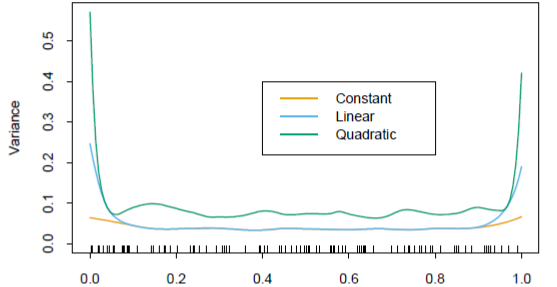
\includegraphics[width=.7\textwidth]{./chap/1chap/3sec/8images/5_linearPoly.PNG}
	\end{center}
	\caption{The variances functions $\norm{l(x)}^{2}$ for local constant, linear and quadratic
	regression, for a metric bandwidth $(\lambda=0.2)$ tri-cube kernel}
	\label{fig:5_linearPol}
\end{figure}
Local linear fits tend to be biased in regions of curvature of the true function, a phenomenon
referred to as \emph{trimming the hills} and \emph{filling the valleys}. Local quadratic regression
is generally able to correct this bias.
\begin{itemize}
	\item \tB{Local linear fits can help bias dramatically at the boundaries at a mode cost
		in variance.} Local quadratic fits do little at the boundaries for bias, but 
		increase the variance a lot.
	\item \tB{Local quadratic fits tend to be most helpful in reducing bias due to curvature
		in the interior of the domain.}
\end{itemize}
\sB{It is not recommended to move from local linear fits at the boundary to local quadratic fits
in the interior. But rather to choose the degree of the fit in function of the application}, if
we are interested in extrapolation then the boundary is of more interest and local linear fits 
are probably more reliable.

\paragraph{Selecting the Width of the Kernel}
\begin{itemize}
	\item For the \tB{\emph{Epanechnikov}} or \emph{tri-cube} kernel with metric width, $\lambda$
		is \sB{the radius of the support region}
	\item For the \tB{\emph{Gaussian}} kernel, $\lambda$ is \sB{the standard deviation}
	\item For the \tB{\emph{k-nearest}} neighborhoods, $\lambda$ is \sB{the number $k$ of nearest
		neighbors}, often expressed as a fraction or span $\frac{k}{N}$ of the total
		training sample.
\end{itemize}
There is a natural bias-variance tradeoff as we change the width of the averaging window:
\begin{itemize}
	\item \tB{If the window is narrow, $\hat{f}(x_{0})$ is an average of a small number of 
		$y_{i}$ close to $x_{0}$, and its variance will be relatively large-close that of
		an individual $y_{i}$.}
	\item If the window is wide, the variance of $\hat{f}(x_{0})$ will be small relative to
		the variance of any $y_{i}$, because of the effect of averaging.
		
\end{itemize}

\paragraph{Local Regression in $\mathbb{R}^{R}$}
Local linear regression will fit a hyperplane locally in $X$, by weighted least squares, with 
weights supplied by a \emph{p-}dimensional kernel.\\
Let $b(X)$ be a vector of polynomial terms in $X$, of maximum degree $d$, 
$
\begin{cases}
	d=0 \Leftarrow b(x) = 1\\
	(d, p)=(1, 2) \Leftarrow b(x) = (1, X_{1}, X_{2})\\
	(d, p)=(2, 2) \Leftarrow b(x) = (1, X_{1}, X_{2}, X_{1}^{2}, X_{2}^{2}, X_{1}X_{2})
\end{cases}
$\\
At each $x_{0}\in\mathbb{R}^{p}$ we solve:
$$ \min\limits_{\beta(x_{0})}\su{{i=1}}{N}K_{\lambda}(x_{0},x_{1})\left(y_{i}-b(x_{i})^{T}\beta(x_{0})\right)^{2}$$ with $K_{\lambda}(x_{0},x_{1})=D\left(\dfrac{\norm{x-x_{0}}}{\lambda}\right)$

\paragraph{Structured Local Regression Models in $\mathbb{R}^{p}$}
\subparagraph{Structured Kernels}
Let be $\bm{A}$ a semi-definite matrix to weigh the different coordinates:
$$ K_{\lambda,A}(x_{0},x)=D\left(\dfrac{(x-x_{0})^{T}\bm{A}(x-x_{0})}{\lambda}\right)$$
If $\bm{A}$ is diagonal, then we can increase or decrease the influence of individual predictors
$X_{j}$ by increasing or decreasing $A_{jj}$

\paragraph{Structured Regression Functions}
We are trying to fit a regression function $\E{Y|X}= f(X_{1}, X_{2},\cdots, X_{p})$ in 
$\mathbb{R}^{p}$. It is natural to consider ANOVA decomposition of the form:
$$ f(X_{1}, X_{2}, \cdots, X_{p}) = \alpha+\su{{j}}{}g_{j}(X_{j})+\su{{k<l}}{}g_{kl}(X_{k},X_{l})
+\cdots$$
and then introduce by eliminating some of the higher-order terms. We then assume the conditionally
linear model:
$$ f(X)=\alpha(Z)+\beta_{1}(Z)X_{1}+\cdots+\beta_{q}(Z)X_{q}$$
For given $Z$, this is a linear model, but each of the  coefficient can vary with $Z$.
$$\min\limits_{\alpha(Z_{0}),\beta(z_{0})}\su{{i=1}}{N}K_{\lambda}(z_{0}, z_{i})\left(y_{i}-
\alpha(z_{0})-x_{1i}\beta_{1}(z_{0})-\cdots-x_{qi}\beta_{q}(z_{0})\right)$$

\subsection{Kernel Density Estimation and Classification}
Kernel density estimation is an unsupervised learning procedure.
\paragraph{Kernel Density Estimation}
Arguing as before, a natural local estimate has the form : \tB{$\hat{f}_{X}(x_{0})=\frac{\#x_{i}\in
\mathcal{N}(x_{0})}{N\lambda}$} where $\mathcal{N}(x_{0})$ is a small metric neighborhood around
$x_{0}$ of width $\lambda$. This estimate is bumpy, and the \sB{smooth \emph{Parzen}} estimate is 
preferred:
$$ \hat{f}_{X}(x_{0}) = \dfrac{1}{N\lambda}\su{{i=1}}{N}K_{\lambda}(x_{0}, x_{i})$$
because it counts observations close to $x_{0}$ with weights that decrease with distance from
$x_{0}$. In this case a popular choice for $K_{\lambda}$ is the Gaussian kernel $K_{\lambda}(
x_{0},x)=\phi\left(\frac{|x-x_{0}|}{\lambda}\right)$

\emph{Python Code}
\begin{python}
import sklearn 
from sklearn.neighbors import KernelDensity

kde = KernelDensity(
  brandwith=0.2
  kernel='gaussian') # or 'tophat','epanechnikov','exponential','linear','cosine'
kde_log_density = kde.score_samples(y)
\end{python}

\paragraph{Kernel Density Classification}
Suppose \sB{for a $J$ class problem we fit non-parametric density estimates $\hat{f}_{j}(X),j\in
\inter{1}{J}$} separately in each the classes, and we also have estimates of the class priors
$\hat{\pi}_{j}$ (usually the sample propositions). Then:
\begin{center}
\enc{$\hat{\mathbb{P}}_{\left\{X=x_{0}\right\}}(G=j)=\dfrac{\hat{\pi}_{j}\hat{f}_{j}(x_{0})}{
\su{{k=1}}{j} \hat{\pi}_{k}\hat{f}_{k}(x_{0})}$}
\end{center}


